353. \begin{figure}[ht!]
\center{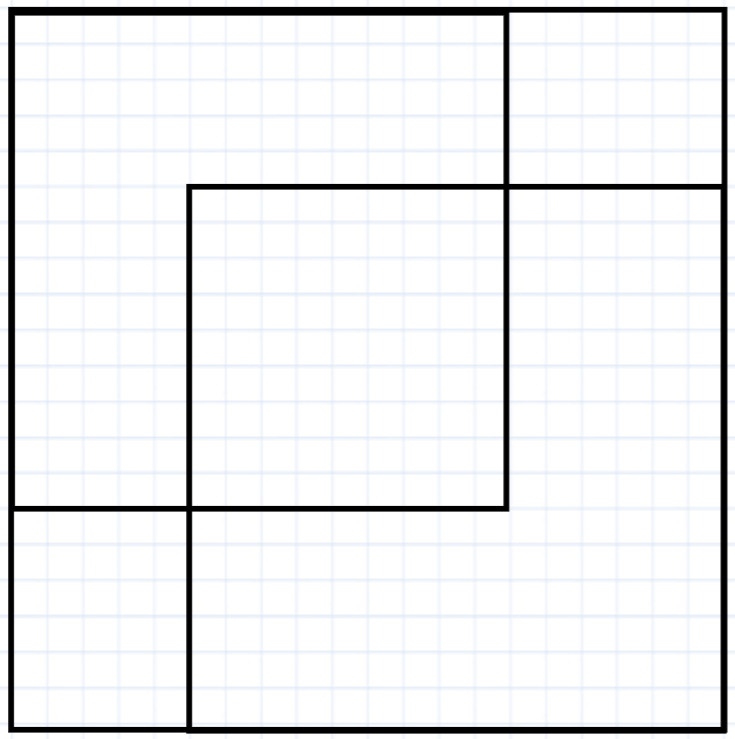
\includegraphics[scale=0.35]{kovr1.png}}
\end{figure}\\
Наименьшая площадь будет покрыта сразу двумя коврами в том случае, когда они лежат в противоположных углах комнаты. В этом случае они вместе покрывают квадрат размером $9\times9$ метров, его площадь равна $9\cdot9=81\text{ м}^2.$\newpage\noindent
